\documentclass[a4paper,12pt]{article}
\usepackage[utf8]{inputenc}
\usepackage[spanish]{babel}
\usepackage{graphicx}
\usepackage{libertine}
\renewcommand\familydefault{\sfdefault}
\usepackage[T1]{fontenc}
\usepackage[colorlinks=true,linkcolor=blue]{hyperref}
\usepackage[framed,numbered,autolinebreaks,useliterate]{mcode}

\parindent = 0mm

\author{Moisés Gautier Gómez}
\title{
\includegraphics[width=10cm]{logo_ugr.png} \\ 
\includegraphics[width=3cm]{fetch.png}\\ Práctica 2 - Teoría de la Señal y Comunicaciones 
}
\date{ }

\begin{document}
\maketitle
Ejercicios
%\lstinputlisting{genexp.m}

\begin{enumerate}
\item Estime los coeficientes de la serie de Fourier de la función:

  $$x(t) = \cos(\omega_{0}t) + (\sin(\omega_{0}t))^2$$

  Para ello haga uso de la siguiente identidad trigonométrica:

  $$e^{j\theta} = \cos(\theta) + j \sin(\theta)$$

  Utilizando MATLAB represente el espectro de magnitud y de fase. ¿Cuántas componentes en frecuencia aparece?.

  Coeficientes:
  $$X(T) = \sum_{n = -\infty}^{\infty} c(n) \cdot e^{j \omega n t}\; ; c(n) = \frac{1}{T} \int_{-\frac{T}{2}}^{\frac{T}{2}} x(t) \cdot e^{-j \omega n t} dt $$

  Con $T$ el periodo de la señal y $\omega$ la frecuencia $(\omega = \frac{2\pi}{T})$.

  Sustituyendo nos quedaría:

  $$c(n) = \frac{1}{T} \int_{-\frac{T}{2}}^{\frac{T}{2}} (\cos(\omega t) + \sin^{2} (\omega t)) \cdot e^{-j \omega n t} dt$$

  Utilizando la identidad trigonométrica siguiente: 
  
  $$ \cos(2\alpha) = 1 - 2\sin^{2}(\alpha)$$

  Obtenemos:
 
  $$ \sin^{2} (\omega t) = \frac{(1 - \cos(2 \omega t))}{2} = \frac{1}{2} - \frac{\cos(2 \omega t)}{2} $$

  Sustituyendo en la integral:

  $$ c(n) = \frac{1}{T} \int_{-\frac{T}{2}}^{\frac{T}{2}} (\cos(\omega t) + \frac{1}{2} - \frac{\cos(2 \omega t)}{2}) \cdot e^{-j \omega n t} dt $$

  Utilizaremos las siguientes igualdades:

  $$ \sin(\alpha) = \frac{e^{i \alpha} - e^{-i \alpha}}{2i} \; \; \; \cos(\alpha) = \frac{e^{i \alpha} + e^{-i \alpha}}{2} $$

  Sustituyendo:
  \begin{eqnarray*}
    c(n) & = & \frac{1}{T} \int_{-\frac{T}{2}}^{\frac{T}{2}} (\frac{e^{j \omega t} + e^{-j \omega t}}{2} + \frac{1}{2} -\frac{e^{2 j \omega t} + e^{-2 j \omega t}}{4}) \cdot e^{-j n \omega t} dt \\ & = & \frac{1}{T} \int_{-\frac{T}{2}}^{\frac{T}{2}} \frac{e^{j \omega t} + e^{-j \omega t}}{2} \cdot e^{-j \omega n t} + \frac{1}{2} \cdot e^{-j \omega n t} - \frac{e^{2 j \omega t} + e^{-2 j \omega t}}{4} \cdot e^{-j \omega n t} dt \\ & = & \frac{1}{T} \int_{-\frac{T}{2}}^{\frac{T}{2}} \frac{e^{j \omega t} \cdot e^{-j \omega n t}}{2} + \frac{e^{-j \omega t} \cdot e^{-j \omega n t}}{2} + \frac{e^{-j \omega n t}}{2} - \lefteqn{\frac{e^{2 j \omega t} \cdot e^{-j \omega n t}}{4}} \\ & & - \frac{e^{-2 j \omega t} \cdot e^{-j \omega n t}}{4} dt
  \end{eqnarray*}

  Por lo que nos queda:

  $$ c(n) = \frac{1}{T} \int_{-\frac{T}{2}}^{\frac{T}{2}} \frac{e^{j \omega t (1-n)}}{2} + \frac{e^{-j \omega t (1+n)}}{2} + \frac{e^{-j \omega n t}}{2} - \frac{e^{j \omega t (2-n)}}{4} - \frac{e^{-j \omega t (2+n)}}{4} dt $$

  Ahora obtenemos el valor de los coeficientes:

  \begin{eqnarray*}
    c(0) & = & \frac{1}{T} \int_{-\frac{T}{2}}^{\frac{T}{2}} \frac{e^{j \omega t}}{2} + \frac{e^{-j \omega t }}{2} + \frac{1}{2} - \frac{e^{j \omega t2}}{4} - \frac{e^{-j \omega t2}}{4} dt \\ & = & \frac{1}{T} \biggl[\frac{e^{j \omega t}}{2 j \omega} + \frac{e^{-j \omega t }}{2 j \omega} + \frac{t}{2} - \frac{e^{j \omega t2}}{8 j \omega} - \frac{e^{-j \omega t2}}{8 j \omega}\biggl]_{-\frac{T}{2}}^{\frac{T}{2}} \\ & = & \frac{1}{T} \lefteqn{\biggl(\frac{e^{j \omega \frac{T}{2}}}{2 j \omega} - \frac{e^{-j \omega \frac{T}{2}}}{2 j \omega} + \frac{T}{4} - \frac{e^{j \omega T}}{8 j \omega} + \frac{e^{-j \omega T}}{8 j \omega} \biggl|_{\frac{T}{2}} } \\ & & - \frac{e^{-j \omega \frac{T}{2}}}{2 j \omega} - \frac{e^{j \omega \frac{T}{2}}}{2 j \omega} - \frac{T}{4} - \frac{e^{-j \omega T}}{8 j \omega} + \frac{e^{j \omega T}}{8 j \omega} \biggl|_{-\frac{T}{2}} \biggl) \\ & = & \frac{1}{T} \lefteqn{\biggl(\frac{e^{j \omega \frac{T}{2}}}{2 j \omega} - \frac{e^{-j \omega \frac{T}{2}}}{2 j \omega} + \frac{T}{4} - \frac{e^{j \omega T}}{8 j \omega} + \frac{e^{-j \omega T}}{8 j \omega} } \\ & & - \frac{e^{-j \omega \frac{T}{2}}}{2 j \omega} + \frac{e^{j \omega \frac{T}{2}}}{2 j \omega} + \frac{T}{4} + \frac{e^{-j \omega T}}{8 j \omega} - \frac{e^{j \omega T}}{8 j \omega} \biggl) \\ & = & \frac{1}{T} \biggl( \frac{2 e^{j \omega \frac{T}{2}}}{2 j \omega} - \frac{2 e^{-j \omega \frac{T}{2}}}{2 j \omega} + \frac{2T}{4} - \frac{2 e^{j \omega T}}{8 j \omega} + \frac{2 e^{-j \omega T}}{8 j \omega} \biggl)
  \end{eqnarray*}

  Utilizando la fórmula de seno y coseno:

  \begin{eqnarray*}
    c(0) & = & \frac{1}{T} \biggl( \frac{2}{\omega} \Bigl(\frac{e^{j \omega \frac{T}{2}} - e^{-j \omega \frac{T}{2}}}{2 j}\Bigl) + \frac{2 T}{4} - \frac{2}{4 \omega} \Bigl(\frac{e^{j \omega T} - e^{-j \omega T}}{2 j}\Bigl) \biggl) \\ & = & \frac{1}{T} \biggl( \frac{2}{\omega} \Bigl(\frac{e^{j \omega \frac{T}{2}} - e^{-j \omega \frac{T}{2}}}{2 j}\Bigl) + \frac{T}{2} - \frac{1}{2 \omega} \Bigl(\frac{e^{j \omega T} - e^{-j \omega T}}{2 j}\Bigl) \biggl) \\ & = & \frac{1}{T} \biggl(\frac{2}{\omega} \sin(\frac{\omega T}{2}) + \frac{T}{2} - \frac{2}{4 \omega} \sin(\omega T) \biggl)
  \end{eqnarray*}

  Fijémonos en lo siguiente:

  $$ \omega T = \bigl( \frac{2 \pi}{T} \bigl) \cdot T \rightarrow\ \omega T = 2 \pi \rightarrow \sin(\omega T) = \sin (2 \pi) = 0 $$

  $$ \frac{\omega T}{2} = \bigl( \frac{2 \pi}{T} \bigl) \cdot \bigl( \frac{T}{2} \bigl) \rightarrow \omega T = \pi \rightarrow \sin(\omega T) = \sin(\pi) = 0 $$

  Por tanto:

  $$ c(0) = \frac{1}{T} \biggl( 0 - \frac{T}{2} + 0 \biggl) = \frac{1}{2} $$

  Siguiente coeficiente:

  \begin{eqnarray*}
    c(1) & = & \frac{1}{T} \int_{-\frac{T}{2}}^{\frac{T}{2}} \frac{1}{2} + \frac{e^{-2 j \omega t}}{2} + \frac{e^{-j \omega t}}{2} - \frac{e^{j \omega t}}{4} - \frac{e^{-3 j \omega t}}{4} dt \\ & = & \frac{1}{T} \biggl[ \frac{t}{2} - \frac{e^{-2 j \omega t}}{4 j \omega} - \frac{e^{-j \omega t}}{2 j \omega} - \frac{e^{j \omega t}}{4 j \omega} + \frac{e^{-3 j \omega t}}{12 j \omega} \biggl]_{-\frac{T}{2}}^{\frac{T}{2}} \\ & = & \lefteqn{\frac{1}{T} \biggl( \frac{T}{4} - \frac{e^{-j \omega t}}{4 j \omega} - \frac{e^{-j \omega \frac{T}{2}}}{2 j \omega} - \frac{e^{j \omega \frac{T}{2}}}{4 j \omega} + \frac{e^{-3 j \omega \frac{T}{2}}}{12 j \omega} \biggl|_{\frac{T}{2}}} \\ & &- \frac{-T}{4} - \frac{e^{j \omega T}}{4 j \omega} - \frac{e^{j \omega \frac{T}{2}}}{2 j \omega} - \frac{e^{-j \omega \frac{T}{2}}}{4 j \omega} + \frac{e^{3 j \omega \frac{T}{2}}}{12 j \omega} \biggl| \biggl) \\ & = & \lefteqn{\frac{1}{T} \biggl( \frac{2 T}{4} + \bigl( \frac{e^{j \omega T}}{4 j \omega} - \frac{e^{-j \omega T}}{4 j \omega} \bigl) + \bigl( \frac{e^{j \omega \frac{T}{2}}}{2 j \omega} - \frac{e^{-j \omega \frac{T}{2}}}{2 j \omega} \bigl)} \\ & &- \bigl( \frac{e^{j \omega \frac{T}{2}}}{4 j \omega} - \frac{e^{-j \omega \frac{T}{2}}}{4 j \omega}\bigl) - \bigl( \frac{e^{3 j \omega \frac{T}{2}}}{12 j \omega} - \frac{e^{-3 j \omega \frac{T}{2}}}{12 j \omega} \bigl) \biggl) \\ & = & \lefteqn{\frac{1}{T} \biggl( \frac{T}{2} + \frac{1}{2 \omega} \bigl( \frac{e^{j \omega T}}{2 j} - \frac{e^{-j \omega T}}{2 j}\bigl) + \frac{1}{w} \bigl( \frac{e^{j \omega \frac{T}{2}}}{2 j} - \frac{e^{-j \omega \frac{T}{2}}}{2 j}\bigl) } \\ & & - \frac{1}{2 \omega} \bigl( \frac{e^{j \omega \frac{T}{2}}}{2 j} - \frac{e^{-j \omega \frac{T}{2}}}{2 j} \bigl) + \frac{1}{6 \omega} \bigl( \frac{e^{3 j \omega \frac{T}{2}}}{2 j} - \frac{e^{-3 j \omega \frac{T}{2}}}{2 j} \bigl) \biggl) \\ & = & \frac{1}{T} \biggl( \frac{T}{2} + \frac{1}{2 \omega} \sin(\omega T) + \frac{1}{\omega} \sin(\frac{\omega T}{2}) + \frac{1}{2 \omega} \sin(\frac{\omega T}{2}) + \frac{1}{6 \omega} \sin(\frac{3 \omega T}{2}) \biggl)
  \end{eqnarray*}

$$ \frac{3 \omega}{2} = 3 (\frac{2 \pi}{T}) \cdot (\frac{T}{2}) \rightarrow \omega T = 2 \pi \rightarrow \sin(\frac{3 \omega T }{2}) = \sin(3 \pi) = 0 $$

$$ c(1) = \frac{1}{2} $$

El coeficiente $-n$ lo sacamos a partir del coeficiente $n$, pues es su conjugado:

$$ c(n)^* = c(-n) $$
$$ c(-1) = \frac{1}{2}$$

Último coeficiente:

\begin{eqnarray*}
c(2) & = & \frac{1}{T} \int_{-\frac{T}{2}}^{\frac{T}{2}} \frac{e^{-j \omega t}}{2} + \frac{e^{-3 \omega 2 t}}{2} + \frac{e^{-j \omega 2 t}}{2} - \frac{1}{4} - \frac{e^{-4 j \omega t}}{4} dt \\ & = & \frac{1}{T} \biggl[ - \frac{e^{-j \omega t}}{2 j \omega} - \frac{e^{-3 j \omega t}}{6 j \omega} - \frac{e^{-2 j \omega t}}{4 j \omega} - \frac{t}{4} + \frac{e^{-4 j \omega t}}{16 j \omega} \biggl]_{-\frac{T}{2}}^{\frac{T}{2}} \\ & = & \lefteqn{\frac{1}{T} \biggl( - \frac{e^{-j \omega \frac{T}{2}}}{2 j \omega} - \frac{e^{-3 j \omega \frac{T}{2}}}{6 j \omega} - \frac{e^{-j \omega T}}{4 j \omega} - \frac{T}{8} + \frac{e^{-2 j \omega T}}{16 j \omega} \biggl|_{\frac{T}{2}}} \\ & & - - \frac{e^{j \omega \frac{T}{2}}}{2 j \omega} - \frac{e^{3 j \omega \frac{T}{2}}}{6 j \omega} + \frac{T}{8} + \frac{e^{2 j \omega T}}{16 j \omega} \biggl|_{-\frac{T}{2}}\biggl) \\ & = & \lefteqn{\frac{1}{T} \biggl( - \frac{e^{-j \omega \frac{T}{2}}}{2 j \omega} - \frac{e^{-3 j \omega \frac{T}{2}}}{6 j \omega} - \frac{e^{-j \omega T}}{4 j \omega} - \frac{T}{8} + \frac{e^{-2 j \omega T}}{16 j \omega}} \\ & & + \frac{e^{j \omega \frac{T}{2}}}{2 j \omega} + \frac{e^{3 j \omega \frac{T}{2}}}{6 j \omega} - \frac{T}{8} - \frac{e^{2 j \omega T}}{16 j \omega} \biggl) \\ & = & \lefteqn{\frac{1}{T} \biggl( \bigl(\frac{e^{j \omega \frac{T}{2}}}{2 j \omega} - \frac{e^{-j \omega \frac{T}{2}}}{2 j \omega}\bigl) + \bigl( \frac{e^{3 j \omega \frac{T}{2}}}{6 j \omega} - \frac{-3 j \omega \frac{T}{2}}{6 j \omega} \bigl)} \\ & & + \bigl( \frac{e^{j \omega T}}{4 j \omega} - \frac{e^{-j \omega T}}{4 j \omega} \bigl) - \frac{2 T}{8} - \bigl( \frac{e^{2 j \omega T}}{16 j \omega} - \frac{e^{-2 j \omega T}}{16 j \omega} \bigl) \biggl) \\ & = & \lefteqn{\frac{1}{T} \biggl( - \frac{T}{4} - \frac{1}{2 \omega} \bigl( \frac{e^{j \omega \frac{T}{2}}}{2 j} - \frac{e^{-j \omega \frac{T}{2}}}{2 j} \bigl) + \frac{1}{3 \omega} \bigl( \frac{e^{3 j \omega \frac{T}{2}}}{2 j} - \frac{e^{-3 j \omega \frac{T}{2}}}{2 j} \bigl) } \\ & & + \frac{1}{2 \omega} \bigl( \frac{e^{j \omega T}}{2 j} - \frac{e^{-j \omega T}}{2 j} \bigl) + \frac{1}{8 \omega} \bigl( \frac{e^{2 j \omega T}}{2 j} - \frac{e^{-2 j \omega T}}{2 j} \bigl) \biggl) \\ & = & \frac{1}{T} \biggl( - \frac{T}{4} + \frac{1}{2 \omega} \sin(\frac{\omega T}{2}) + \frac{1}{3 \omega} \sin(\frac{3 \omega T}{2}) + \frac{1}{2 \omega} \sin(\omega T) + \frac{1}{8 \omega} \sin(2 \omega T) \biggl)
\end{eqnarray*}

$$ c(2) = - \frac{1}{4} $$
$$ c(-2) = - \frac{1}{4} $$

Si seguimos calculando, aparecen nada más que exponenciales, lo que implica que habrá ceros. La señal queda de la siguiente forma:

$$ X(t) = \frac{1}{2} + \frac{1}{2} e^{i \omega t} - \frac{1}{4} e^{2 i \omega t} + \frac{1}{2} e^{-i \omega t} - \frac{1}{4} e^{-2 i \omega t} $$

Utilizando MATLAB represente el espectro de magnitud y de fase. ¿Cuántas componentes en frecuencia aparecen?.

El espectro de magnitud lo representaremos calculando el módulo de los coeficientes, con la función $abs$ (para calcular el valor absoluto). Los módulos de los coeficientes son su propio valor, pues son números reales. El espectro de fase lo calcularemos con la función $angle$, dado que todos nuestro coeficientes son cero, pues no existe parte imaginaria.

\lstinputlisting{../ejercicio-1.m}
\begin{center}
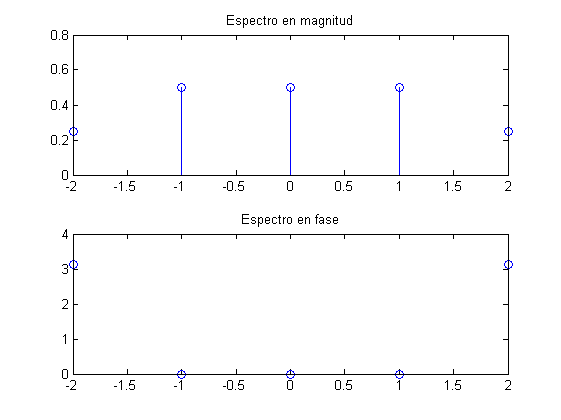
\includegraphics[width=.8 \textwidth]{../ejercicio-1.png}
\end{center}

Aparecen 5 componentes en frecuencia: $0, \omega, -\omega, 2 \omega, -2 \omega $

\item Determinar y representar los coeficientes de la serie de Fourier de un tren de impulsos.

Para calcular los coeficientes aplicamos la fórmula de la serie de Fourier.

$X(T) = \sum_{n = - \infty}^{\infty} c(n) \cdot e^{j \omega n t}$ \quad \quad \quad $c(n) = \frac{1}{T} \int_{-\frac{T}{2}}^{\frac{T}{2}} x(t) \cdot e^{-j \omega n t} dt$ 

$c(n) = \frac{1}{T} \int_{-\frac{T}{2}}^{\frac{T}{2}} \sum_{k = -\infty}^{\infty} A \delta(t - kT) \cdot e^{-j \omega n t} dt$

Si nos damos cuenta, solo tenemos un impulso, ya que integramos entre $\frac{-T}{2}$ y $\frac{T}{2}$,

$c(n) = \frac{1}{T} \int_{-\frac{T}{2}}^{\frac{T}{2}} A \delta(t) \cdot e^{-j \omega n t} dt = \frac{A}{T} \int_{-\frac{T}{2}}^{\frac{T}{2}} \delta(t) \cdot e^{-j \omega n t} dt$

Según las propiedades de la función delta: $\int \delta(t - t_o) \cdot x(t) dt = x(t_0)$

Por tanto: $\int \delta(t) \cdot x(t) dt = x(0)$

Sustituyendo:

$$ c(n) = \frac{A}{T} \int_{-\frac{T}{2}}^{\frac{T}{2}} \delta(t) \cdot e^{-j \omega n t} dt = \frac{A}{T} e^{-j \omega 0 t} = \frac{A}{T} $$

La serie de Fourier nos queda con todos los coeficientes iguales:

$$ X(T) = \sum_{n = -\infty}^{\infty} \frac{A}{T} \cdot e^{j \omega n t} = \frac{A}{T} \sum_{n = -\infty}^{\infty} e^{j \omega n t} $$

Para la representación mediante MATLAB he seleccionado un tren de impulsos de periodo 5 y amplitud 5.

\lstinputlisting{../ejercicio-2.m}
\begin{center}
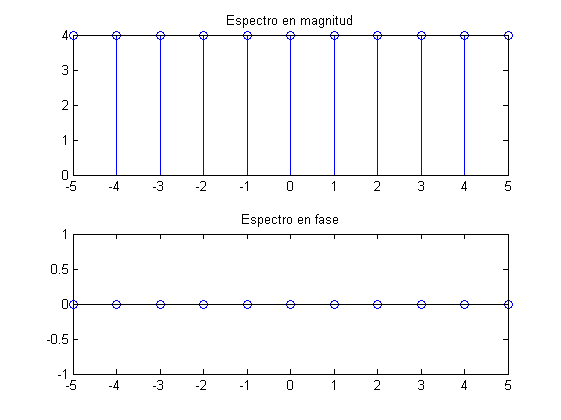
\includegraphics[width=.8 \textwidth]{../ejercicio-2.png}
\end{center}
\item Realice una función MATLAB que determine y represente el espectro de magnitud de un tren periódico de pulsos cuadrado de amplitud A, anchura d y periodo T.

Un impulso cuadrado se representa con la siguiente expresión matemática:

\begin{displaymath}
\prod(t) = \left\{ \begin{array}{ll}
1 & \frac{-T}{2} \leq t \leq \frac{T}{2} \\
0 & |t| > \frac{T}{2} \\
\end{array}
\right.
\end{displaymath}

Un tren de impulsos cuadrados, de amplitud $A$, periodo $T$ y de anchura $d$, podemos representarlo como:

\begin{displaymath}
x(t) = \left\{ \begin{array}{ll}
A & kT \leq t \leq kT +d \\
0 & |t| > kT + d \\
\end{array}
\right.
\end{displaymath}

\lstinputlisting{../trenImpulsos.m}

Para la representación del tren de impulsos he escogido un tren de amplitud 5, anchura 3 y periodo 5, para el intervalo $[-30,30]$:

\lstinputlisting{../ejercicio-3-a.m}

\begin{center}
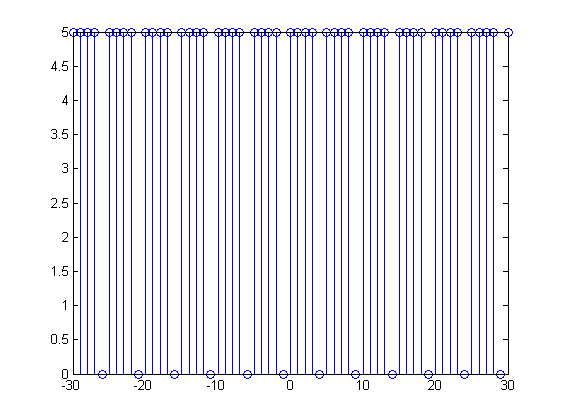
\includegraphics[width=.8 \textwidth]{../ejercicio-3-a.png}
\end{center}

Ahora calculo los coeficientes correspondientes a la serie de esta señal y su representación:

\lstinputlisting{../Fourier.m}

\lstinputlisting{../ejercicio-3-b.m}

\begin{center}
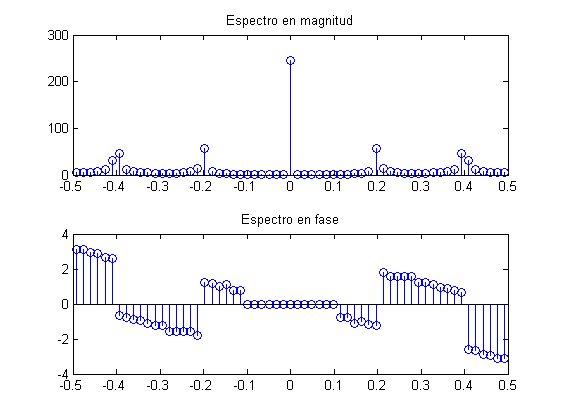
\includegraphics[width=.9 \textwidth]{../ejercicio-3-b.png}
\end{center}

\item Partiendo de la expresión de la sinusoide de tiempo continuo, escriba una función MATLAB que obtenga muestras de $s(t)$ para crear con ellas una función de tiempo discreto de longitud finita. Esta función requiere seis entradas: tres para los parámetros de la señal, dos para los tiempos de comienzo y final de muestreo y uno para la frecuencia de muestreo (en hercios). Para la función que corresponde a la señal de tiempo continuo definida, considere que las unidades de comienzo y final son segundos y no los índices de las muestras. Realice la representación de la señal resultante para tres frecuencias de muestreo distintas.

La expresión de la sinusoide de tiempo continuo es la siguiente:

$$ s(t) = A \cos(2 \pi f t + \theta) $$

Así pues vamos a definir una función en MATLAB para la expresión anteriormente citada:

\lstinputlisting{../sinusoide.m}

Ahora haremos una representación gráfica de la función para unos valores de amplitud 4, periodo 5 con un rango de valores entre $[-5,5]$:

\lstinputlisting{../ejercicio-4-a.m}

\begin{center}
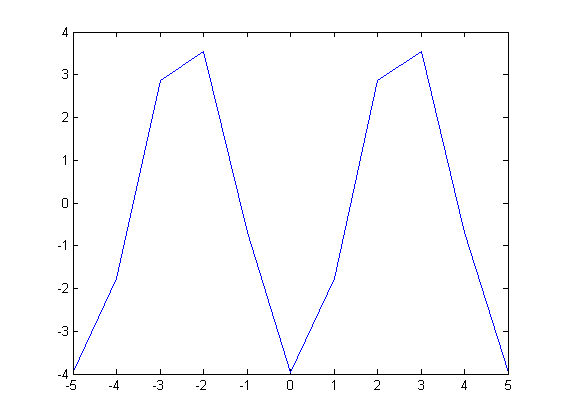
\includegraphics[width=.9 \textwidth]{../ejercicio-4-a-2.png}
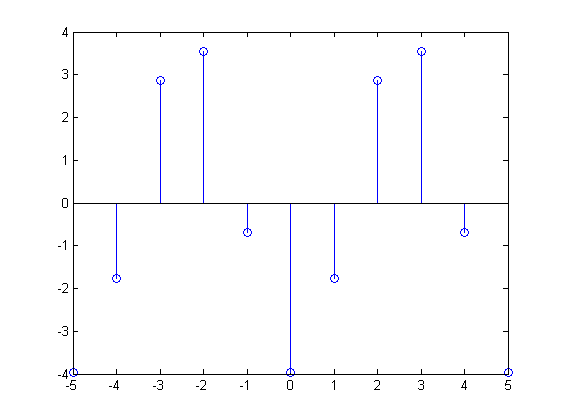
\includegraphics[width=.9 \textwidth]{../ejercicio-4-a-1.png}
\end{center}

La frecuencia máxima para esta función es:

$$ \omega = \frac{2 \pi}{T} = \frac{2 \pi}{T} \approx 1.25 Hz$$

Y ahora usando el teorema de muestreo definimos la siguiente función en MATLAB:

\lstinputlisting{../muestreo.m}

Usamos dicha función para distintas frecuencias de muestreo (para fs = 0,5; 1,25; 3,00):

\lstinputlisting{../ejercicio-4-b.m}

\begin{center}
$fs = 0,5$
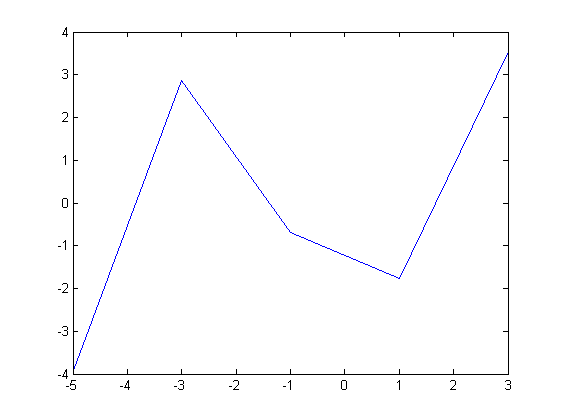
\includegraphics[width=.9 \textwidth]{../ejercicio-4-b-2.png}
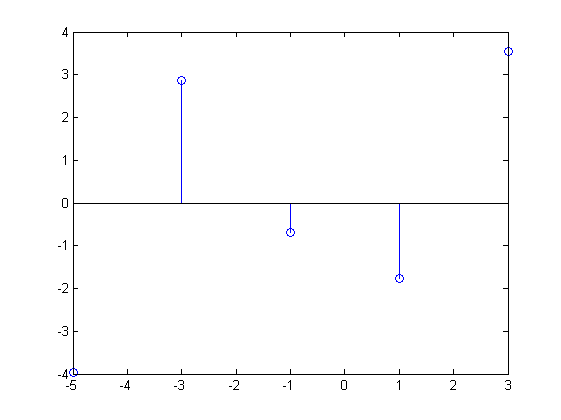
\includegraphics[width=.9 \textwidth]{../ejercicio-4-b-1.png}
\end{center}

\begin{center}
$fs = 1,25$
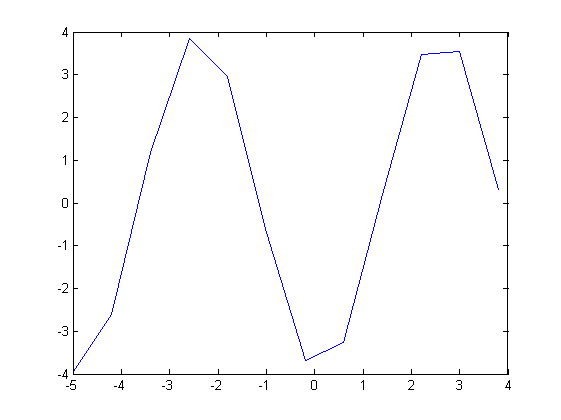
\includegraphics[width=.9 \textwidth]{../ejercicio-4-b-4.png}
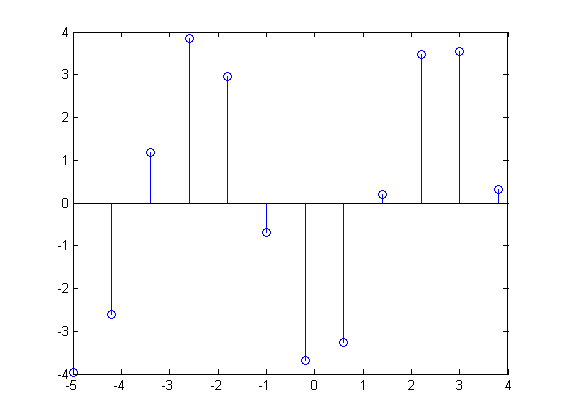
\includegraphics[width=.9 \textwidth]{../ejercicio-4-b-3.png}
\end{center}

\begin{center}
$fs = 3,00$
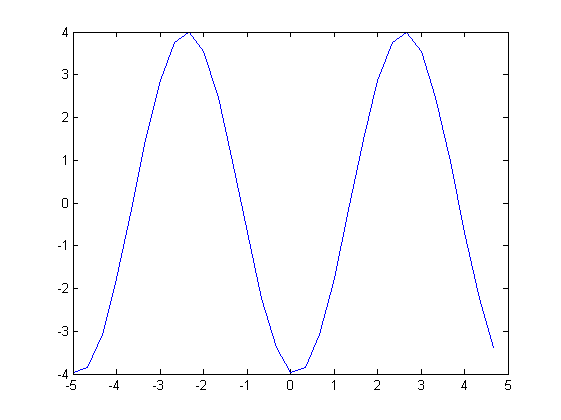
\includegraphics[width=.9 \textwidth]{../ejercicio-4-b-6.png}
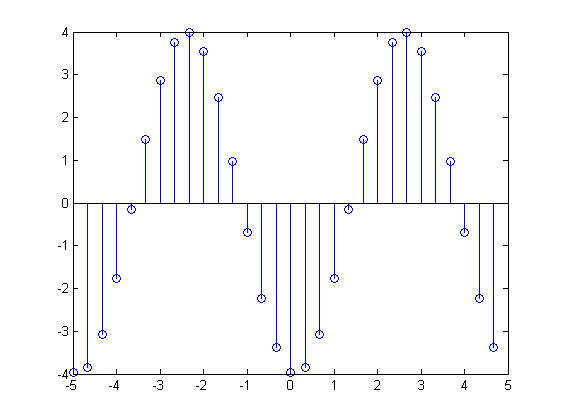
\includegraphics[width=.9 \textwidth]{../ejercicio-4-b-5.png}
\end{center}

\item Obtenga y represente gráficamente el espectro de módulo de las señales muestreadas generadas en el apartado anterior. Discuta los resultados obtenidos.

Ahora lo que tenemos que aplicar es la función de Fourier sobre nuestro vector resultante del muestreo para ver el espectro de la señal resultante en magnitud y en fase. Seleccionamos en el mismo orden las señales generadas anteriormente, es decir, $fs = 0,5; 1,25; 3,00$:

\lstinputlisting{../ejercicio-5.m}

\begin{center}
$fs = 0,5$
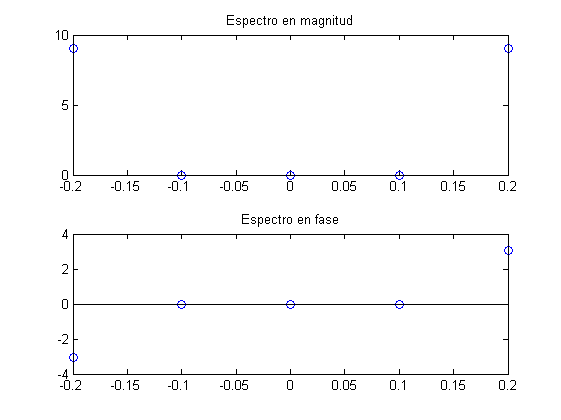
\includegraphics[width=.9 \textwidth]{../ejercicio-5-a.png}
\end{center}

\begin{center}
$fs = 1,25$
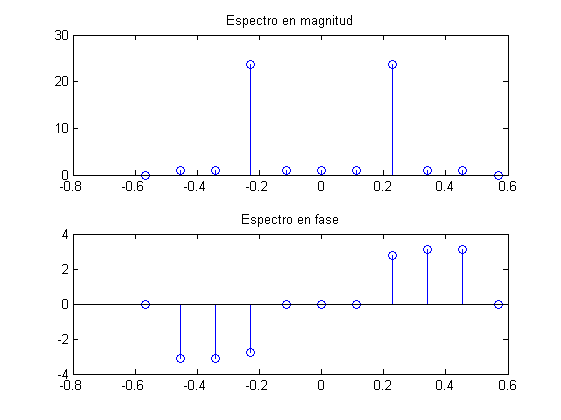
\includegraphics[width=.9 \textwidth]{../ejercicio-5-b.png}
\end{center}

\vspace*{.25in}{
\begin{center}
$fs = 3,00$
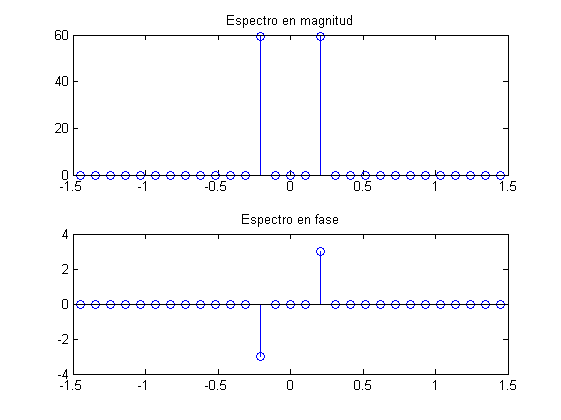
\includegraphics[width=.9 \textwidth]{../ejercicio-5-c.png}
\end{center}}

La mínima frecuencia (teórica) de muestreo $f$, necesaria para conseguir recuperar la señal original se conoce como frecuencia de Nyquist ($f_N$), y es igual al doble de la frecuencia máxima ($f$) que contenga la señal a muestrear: $f_N = 2 f$. Por lo tanto, para realizar el muestreo de forma correcta se debe cumplir lo que se conoce como criterio de Nyquist: $f_{S}^{3} f_N$ , es decir: $f_{S}^{3} 2 f$.

La señal original es un coseno de frecuencia $f = 1,25 Hz$ y primero se muestreó a $f_S = 0,5 Hz$. No se cumple el criterio presentado antes porque $f_s < f_N$, donde recordemos que $f_N = 2 \cdot f = 2 \cdot 1,25 = 2,5 Hz$ que es inferior a $f_s = 0,5$. De ahí que no consigamos recuperar la señal original sino otra de menor frecuencia. Esta señal recuperada debe cumplir el criterio de Nyquist, por lo que su frecuencia $f$ debe ser tal que $2 f \leq f_s$. Dado que la frecuencia de muestreo era $f_s = 0,5 Hz$ resulta $f \leq 0,25 Hz$.

Si aumentamos la frecuencia de muestreo a $f_s = 3 Hz$, ahora sí se cumple el criterio de Nyquist porqué $f_s^3 f_N$ , esto es, $3^3\ 2,5$, por lo que el muestreo se realiza de forma correcta y podemos recuperar la señal original.

Finalmente, en el caso en el que $f_s = f_N$, las muestras coinciden exactamente en los mínimos y máximos de la señal, de forma que no perdemos información sobre ésta.

\end{enumerate}
\end{document}

